% TODO: make it clear that if data models have IVORNs, it's those people should look for, and *never* DM names, which are purely informative for IVOA DMs.

\documentclass{ivoa}
\input tthdefs

\usepackage{listings}
\lstloadlanguages{XML}
\lstset{flexiblecolumns=true,tagstyle=\ttfamily,
showstringspaces=False}

\ivoagroup{Registry}

\author[http://www.ivoa.net/cgi-bin/twiki/bin/view/IVOA/MarkusDemleitner]{Markus
Demleitner}
\author[http://www.ivoa.net/cgi-bin/twiki/bin/view/IVOA/PatrickDowler]{Patrick
Dowler}
\author[http://www.ivoa.net/cgi-bin/twiki/bin/view/IVOA/RayPlante]{Ray
Plante}
\author[http://www.ivoa.net/cgi-bin/twiki/bin/view/IVOA/GuyRixon]{Guy
Rixon}
\author[http://www.ivoa.net/cgi-bin/twiki/bin/view/IVOA/MarkTaylor]{Mark
Taylor}

\editor{Markus Demleitner}

\previousversion[http://www.ivoa.net/documents/TAPRegExt/20120827/]{REC-1.0}
\previousversion[http://www.ivoa.net/Documents/TAPRegExt/20120208]{PR-20110727}

\title{TAPRegExt}

\begin{document}

\begin{abstract}
This document describes an XML encoding standard for metadata about
services implementing the table access protocol TAP \citep{std:TAP}, referred to as TAPRegExt.  Instance documents are
part of the service's registry record or can be obtained from the service
itself.  They deliver information to both humans and software on the languages,
output formats, and upload methods supported by the service, as well as data
models implemented by the exposed tables, optional language features,
and certain limits enforced by the service.
\end{abstract}


\section{Introduction}

\label{introduction}

The Table Access Protocol TAP \citep{std:TAP} allows
VO clients to send queries to remote database servers and receive the
results in standard formats.  In addition, it defines means to discover
database schemata on the remote side, to upload data from the local disk
or third-party hosts, and more.  TAP builds upon a variety of other
standards, premier among which is the Universal Worker Service 
\citep{std:UWS}, which describes how client and server
can negotiate the execution of a query and the retrieval of results
without having to maintain a continuous connection.

To accommodate a wide variety of requirements, the TAP specification
offers implementors many choices on optional features, resource limits, or
locally defined functionality.  One purpose of TAPRegExt is to allow the
service to communicate such choices to remote clients using the mechanisms
laid down in the VO Service Interfaces standard \citep{std:VOSI}

Clients also need to discover TAP services offering certain kinds of data.
Central to this is the concept of a registry in which resources can be
described and consequently discovered by users and applications in the VO.
Registries receive resource descriptions as defined in the IVOA standard 
\citep{std:VOR}. In this schema, support for 
a standard service protocol is described as a service's capability; the
associated metadata is contained within the service resource description's
\texttt{<capability>} element.

TAPRegExt defines this capability element for TAP services.  In the context
of registering TAP services, an important role filled by TAPRegExt is the 
communication of supported data models to the registry.


\subsection{TAPRegExt within the VO Architecture}

\label{architecture}

\begin{figure}[thm]
\begin{center}
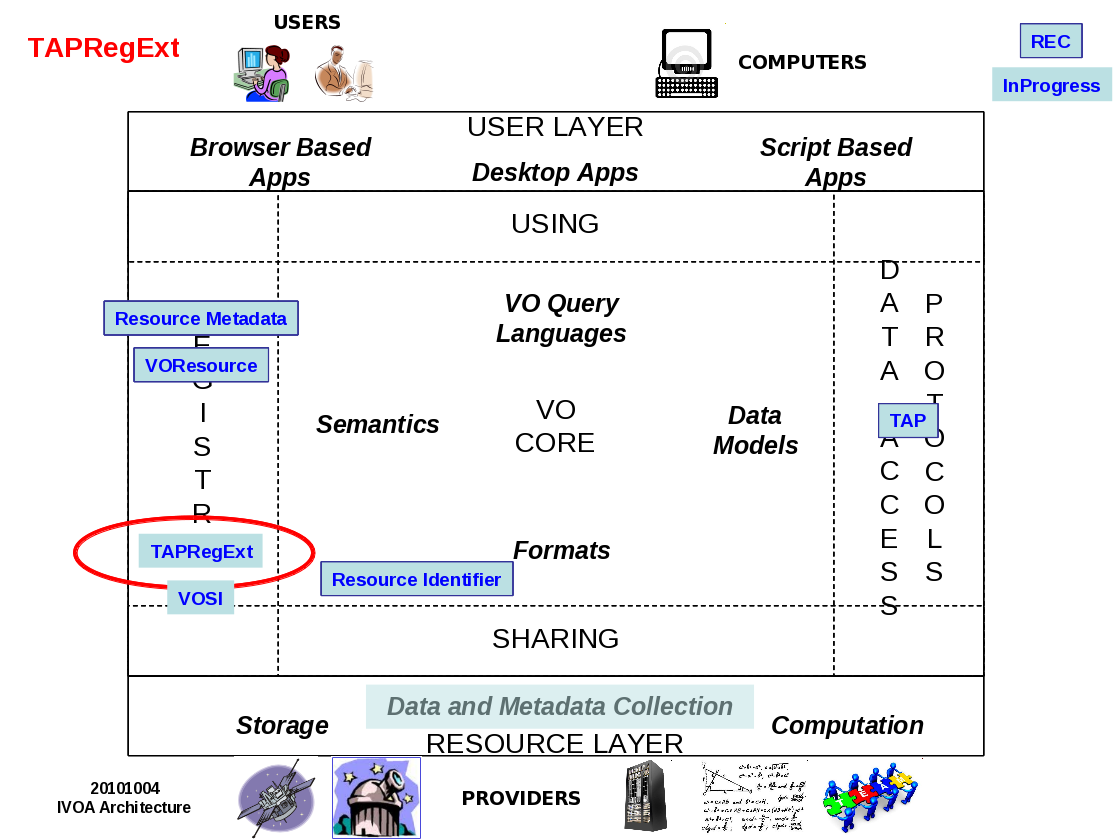
\includegraphics[width=0.9\textwidth]{TAPRegExt-arch.png}
\end{center}
\caption{IVOA Architecture diagram with TAPRegExt and
the related standards marked up}
\label{fig:arch}
\end{figure}

This specification directly relates to other IVOA standards in the following
ways:


\begin{description}
\item[VOResource, v1.03 \citep{std:VOR}] Descriptions of services that support TAP are encoded
using the VOResource XML schema. TAPRegExt is an extension 
of the VOResource core schema.
\item[TAP, v1.0 \citep{std:TAP}]The TAP standard defines some of the concepts that TAPRegExt
deals with. The TAP standard document indirectly
refers to this document in the specification of its capabilities endpoint.
\item[UWS, v1.0 \citep{std:UWS}]The UWS standard describes additional parameters the choices 
of which are communicated using TAPRegExt.
\item[StandardsRegExt \citep{std:STDREGEXT}] TAPRegExt uses the StandardKeyEnumeration mechanism introduced
in StandardsRegExt to define controlled vocabularies.

\end{description}

This standard also relates to other IVOA standards:


\begin{description}
\item[IVOA Support Interfaces, v1.0 \citep{std:VOSI}] VOSI describes the standard interfaces to discover metadata about
services; this document defines the response TAP services should
provide on the \texttt{capabilities} endpoint described by VOSI.
\item[IVOA defined data models]Data models specified by the IVOA can define the structure of
database tables holding instances of those data models.
The first example of such a definition is given by
\citep{std:OBSCORE}{[ObsCore]}.  Services providing
access to such tables
can declare that fact within TAPRegExt instance documents.

\end{description}


% HTML section ends

% subsection architecture

% HTML section ends

% section introduction

% HTML section start

\section{The Extension}

\label{taextension}

\subsection{The Schema Namespace and Location}

\label{nsloc}

The namespace associated with TAPRegExt VOResource extensions is
\texttt{http://www.ivoa.net/xml/TAPRegExt/v1.0}.  
Just like the namespace URI for the VOResource schema, the
TAPRegExt namespace URI can be interpreted as a URL.  Resolving it
returns the XML schema document (given in \ref{fullschema})
that defines the TAPRegExt schema.

Authors of VOResource instance documents may choose to
provide a location for the VOResource XML schema document and its
extensions using the
\xmlel{xsi:schemaLocation} attribute.  
While generators are
free to provide any schema location (e.g., a local mirror), this specification
recommends using the TAPRegExt namespace URI as its location URL
(as illustrated in the example above), as in,


\begin{verbatim}
xsi:schemaLocation="http://www.ivoa.net/xml/TAPRegExt/v1.0
                    http://www.ivoa.net/xml/TAPRegExt/v1.0"
\end{verbatim}

Note that you must give the \texttt{xsi:schemaLocation} of
the TAPRegExt schema when the capability defined here is part of a published
registry resource record as per the IVOA Registry Interface standard 
\citep{std:RI1}.  This does not apply to the use
in a TAP server's capabilities endpoint.


\subsection{Declaring Instantiated Data Models}

\label{dms}

The IVOA defines certain data models that can be instantiated in database
tables exposed by a TAP service.  This allows a query built exclusively
on a data model or a set of data models to work on all TAP services exposing
tables instantiating the data model(s).

In TAPRegExt, a data model is identified by its IVOA identifier
\citep{std:VOID}.  The first example for such a data model is ObsCore
\citep{ref:OBSCORE}.


\subsection{Languages Supported}

\label{langs}

TAP services may offer a variety of query languages.  In TAPRegExt, the
\texttt{language} element allows the communication of what languages are
available on a service.  TAP defines values of the \texttt{LANG} parameter
to have either the form \texttt{<name>-<version>} or the form
\texttt{<name>}, where the latter form leaves the choice of the
version to the server.  Therefore, a language is defined using a name and one
or more versions.

The recommended way to associate larger amounts of documentation with a
language entry in a capability element is via registration of the language
using the mechanisms defined in \citep{std:STDREGEXT} and associating
the registry record with the language element through the latter's ivo-id
attribute.  The IVOID for the only language mandatory for TAP services,
ADQL 2.0, is 
\nolinkurl{ivo://ivoa.net/std/ADQL#v2.0}.
.

The type of the \texttt{ivo-id} attribute on version is 
\texttt{xs:anyURI} as opposed to \texttt{vr:IdentifierURI} since
the latter does not allow frament identifiers. 
The description constrains the value to be an
IVORN, though.  The same reasoning applies to the \texttt{ivo-id}
attributes of \texttt{outputFormat} and \texttt{uploadMethod}.

Query languages may support optional features.  For ADQL, the most prominent
of those are user-defined functions, i.e., functions not defined in the language
standard but added by the operators of the service, and geometry functions.
Such optional features may be communicated to the service client in
\texttt{tr:languageFeatures} elements.  

Each such list is labelled with a \texttt{type} attribute
indicating the type of language option being described.
This string should be an IVORN whose semantics in this context,
along with the semantics of the content of its descendant 
\texttt{feature/form} elements,
can be documented in association with the language in question.

TAPRegExt itself defines the following feature types:


\begin{description}
\item[\nolinkurl{ivo://ivoa.net/std/TAPRegExt\#features-udf}] Each feature declares a user-defined ADQL (or similar) function supported.
    The content of the \texttt{form} element
    must be the signature of the function, written to match the
    \texttt{signature} nonterminal in the following grammar:


\begin{verbatim}
signature ::= <funcname> <arglist> "->" <type_name>
funcname  ::= <regular_identifier>
arglist   ::= "(" <arg> { "," <arg> } ")"
arg       ::= <regular_identifier> <type_name>
\end{verbatim}

The \texttt{type\_name} nonterminal is not defined by the ADQL
		grammar. For the purposes of TAPRegExt, it is sufficient to assume
		it expands to "some sort of SQL type specifier" (which may
		include spaces and parentheses).  For an enumeration of common types
		in ADQL, refer to the last column of the table in section 2.5 of 
		\citep{std:TAP}.

Example:


\begin{lstlisting}[language=XML]
<languageFeatures type="ivo://ivoa.net/std/TAPRegExt#features-udf">
  <feature>
    <form>match(pattern TEXT, string TEXT) -> INTEGER</form>
    <description>
      match returns 1 if the POSIX regular expression pattern 
      matches anything in string, 0 otherwise.
    </description>
  </feature>
</languageFeatures>
\end{lstlisting}


\item[\nolinkurl{ivo://ivoa.net/std/TAPRegExt\#features-adqlgeo}] Each feature declares support for one of the geometry functions 
		defined by ADQL
    (support for these functions is in general optional for ADQL
    implementations, though TAP imposes some constraints on what 
    combinations of support are permitted).

The signature of these functions, where supported, is fixed by ADQL;
    the content of the \texttt{form} element
    is just the name of the function.

Example:


\begin{lstlisting}[language=XML]
<feature>
  <form>CONTAINS</form>
</feature>
\end{lstlisting}



\end{description}


\subsection{Output Formats}

\label{outforms}

A TAP service may offer a variety of output formats.
What output formats are available is defined using
\texttt{outputFormat} elements.   They 
declare a MIME type \citep{std:RFC2045} as well
as aliases (the shorthand forms the server also accepts in the 
FORMAT parameter).  If desired, the format can be further described with an
IVORN in the ivo-id attribute; TAPRegExt provides keys for some variants of
VOTables which are not interoperably distinguishable by their MIME types so far:


\begin{description}
\item[\texttt{output-votable-td}]A VOTable in which all DATA elements contain a TABLEDATA element
\item[\texttt{output-votable-binary}]A VOTable in which all DATA elements contain a STREAM element
	with a BINARY child
\item[\texttt{output-votable-binary2}]A VOTable in which all DATA elements contain a STREAM element
	with a child of the yet-to-be-defined BINARY2 VOTable element
\end{description}


\subsection{Upload Methods}

\label{uploadmethods}

TAP services should allow the upload of VOTables.  They can support
various methods to do this: HTTP upload, retrieval by URL, but also VOSpace
or possibly retrieval using Grid protocols.  Since an actual specification
of the details of such protocols is far beyond the scope of a registry
document and probably would not benefit clients anyway, the upload
methods are given as IVORNs.

IVORNs for the standard upload methods are provided within the
resource record
\texttt{ivo://ivoa.net/std/TAPRegExt}.  
The IVORNs are built by using the keys as fragment identifiers within the 
TAPRegExt IVORN.

It is permitted to register upload methods under authorities other than
ivoa.net.
The registry records can then provide more in-depth information. For
the upload methods defined in the TAP specification, however, 
the IVORNs of the keys in the TAPRegExt resource record must be used to enable
clients to identify supported methods using string comparisons.

This document defines the following protocol identifiers:


\begin{itemize}

\item \texttt{upload-inline} -- HTTP upload as per section 2.5.2 of 
\citep{std:TAP}.{}

\item \texttt{upload-http} -- retrieval from an http URL.{}

\item \texttt{upload-https} -- retrieval from an https URL.{}

\item \texttt{upload-ftp} -- retrieval from an ftp URL.{}

\end{itemize}

Thus, a service offering upload by retrieving from ftp and http URLs
would say:


\begin{lstlisting}[language=XML]
  <uploadMethod ivo-id="ivo://ivoa.net/std/TAPRegExt#upload-http"/>
  <uploadMethod ivo-id="ivo://ivoa.net/std/TAPRegExt#upload-ftp"/>
\end{lstlisting}

\subsection{Resource Limits}

\label{reslimits}

TAP services usually impose certain limits on resource usage by clients,
e.g., a maximum run time per query, or a maximum number of rows in the result
set.  Services assign such limits to newly created jobs and may
allow raising the limits by means of queries or query parameters (e.g., the
size of the result set is limited by the \texttt{MAXREC} parameter, whereas
the date of job destruction may be changed by posting to the
\texttt{destruction} parameter).  Services may put some limit to how
far the resource limitations may be raised.

TAPRegExt's capabilities element allows the declaration of such limits.
These declarations are primarily intended for human consumption and should give
conservative guidelines.  Thus, the operators of a service implementing a
complex, possibly dynamic limits policy should give lower estimates here.

If a service supports authentication and has different
limits depending on what user is authenticated, it should return the
limits applying to the logged user.

The resource limits applying to newly created jobs are given in
\texttt{default} elements, the limits beyond which users cannot
raise the limits are given in \texttt{hard} elements.

Note that the absence of a specification of limits does not imply that
no limits are enforced.


\subsubsection{Limits on Time}
Limits on TimeThis document defines two time-like resource limits:


\begin{itemize}

\item \texttt{retentionPeriod} -- the time from job creation until
		\texttt{destruction}.{}

\item \texttt{executionDuration} -- the maximal run time given to
		a query.{}

\end{itemize}
All values in time-like limits are given in seconds.  Both 
\texttt{retentionPeriod} and \texttt{executionDuration} are of type
\texttt{tr:TimeLimits}.


\subsubsection{Limits on Data}
Limits on DataLimits on data are expressed much like time limits in that they give
\texttt{default} and a \texttt{hard} value as well.  
Both those values have a unit attribute that can either be \texttt{byte}
or \texttt{row} for data limits.

This document defines two resource limits on data:


\begin{itemize}

\item \texttt{outputLimit} -- if \texttt{unit} is \texttt{row} here,
the \texttt{default} gives the
value of TAP's \texttt{MAXREC} parameter the service will use when none
is specified.{}

\item \texttt{uploadLimit} -- the maximum size of uploads.  This 
is not a TAP adjustable parameter.  The \texttt{default} value
advises clients about the server's wishes as to a limit above which
some sort of acknowledgement should be requested from the user.  The 
\texttt{hard} limit gives the maximum size of an upload to the 
server.{}

\end{itemize}
Data limits are defined using the \texttt{tr:DataLimits}
and \texttt{tr:DataLimit} types:


\subsection{The Capability Record}

\label{caprec}

Using the types defined above, the 
\texttt{tr:TableAccess} type can be defined.  Note that
it is a type, not a (global) element.  In instance documents, you
will typically place it in a capability element with an explicit
type specification, like this:


\begin{lstlisting}[language=XML]
  <capability 
    xmlns:tr="http://www.ivoa.net/xml/TAP/v1.0" 
    xmlns:xsi="http://www.w3.org/2001/XMLSchema-instance" 
    standardID="ivo://ivoa.net/std/TAP" 
    xsi:type="tr:TableAccess">
    ...
\end{lstlisting}

By restriction from VOResource's \texttt{vr:Capability}, the 
\texttt{standardID} attribute of \texttt{tr:TableAccess}-typed 
capabilities is fixed to \texttt{ivo://ivoa.net/std/TAP} in this version.
This string can be used to locate TAP services in the registry.


\appendix


\section{The Full Schema}

\label{fullschem}

\lstinputlisting[language=XML,basicstyle=\footnotesize]{TAPRegExt-v1.0.xsd}

\section{Example Document}

\label{appB}

As an example, here is an instance document as it might be 
part of a response from a VOSI capability endpoint or embedded 
within a VOResource record:

Note that the encoding parameter in the MIME type given for the output format
\nolinkurl{ivo://ivoa.net/std/TAPRegEXT\#output-votable-td} in the example is not
endorsed by IVOA.  Within the example, it represents a local convention.


\lstinputlisting[language=XML,basicstyle=\footnotesize]{sample.xml}

\section{Changes from Previous Versions}

\label{changes}

\section{Changes from REC-1.0}

\label{changes-rec-1.0}

\begin{itemize}

\item Fixed obscore data model URI to what the obscore standard specifies.{}

\item dataModel/@ivo-id is now typed xs:anyURI
to allow fragment identifiers on it.{}

\end{itemize}

\section{Changes from WD-20110127}

\label{changes-20110127}

\begin{itemize}

\item userDefinedFunction was generalized to feature within languageFeatures.{}

\item The uploadmethods StandardKeyEnumeration was replaced by a
resource record for TAPRegExt as a whole.  This now includes keys of output
formats and features as well; therefore, upload method names in their new
IVORNs are prefixed with upload-{}

\item Schema version was bumped to 1.0 (yes, we indulge in unversioned
schema changes before this becomes REC).{}

\item uploadLimit interpretation was changed: The default limit is now
"advisory" and to be interpreted as such by clients, the hard limit
is what is actually required by the server.{}

\item There's now an optional ivo-id attribute on the version element
within language.{}

\item There's now an optional ivo-id attribute on output formats.{}

\end{itemize}

\section{Changes from WD-20110727}

\label{changes-20110727}

\begin{itemize}

\item The namespace in the schema is now \nolinkurl{http://www.ivoa.net/xml/TAPRegExt/v1.0} consistent with what has already been stated in the text.{}

\item The IVORN for ADQL is now \nolinkurl{ivo://ivoa.net/std/ADQL\#v2.0}; it is defined here to be in ADQL's record since we do not want to wait for the ADQL standard to be fixed, but ADQL versioning should really not be done here, so a TAPRegExt IVORN is out of the question.{}

\item The IVORN of the TAPRegExt standard is now \texttt{ivo://ivoa.net/std/TAPRegExt} to conform with other standard IVORNs.  Unfortunately, this changes
all other IVORNs dependent on this.{}

\item We now allow AnyURI on the ivo-id of language to allow fragment identifiers as, e.g., in ADQL.{}

\end{itemize}


\section{Changes from PR-20120812}

\label{changes-20120208}

\begin{itemize}

\item Fixed units in limits to "row" and "byte".{}

\end{itemize}

\section{Changes from REC-1.0}

\label{changes-v1.0}

\begin{itemize}

\item Migrated to ivoatex
\item Fixed the IVORN of the obscore data model in the example.{}

\end{itemize}

\bibliography{ivoatex/ivoabib}

\end{document}
